\chapter{Introduction and Opening Remarks}
\label{sec:intro}

Lyman-$\alpha$ "blobs" (LABs) are an enigmatic class of objects first discovered roughly $2$ decades ago \citep{Fynbo1999,Steidel2000}, and are characterized by copious Ly$\alpha$ luminosity, as well as their large spatial extent.
While there are no hard constraints on the definition of a blob, the majority of blobs have luminosities $L_{\rm{Ly}\alpha} > 10^{43}$ erg/s, and spatial extents that exceed $\sim50$ kpc in radius.
We will discuss this definition in more detail shortly.

Since their discovery, the dominant source of power in these objects has been under debate, and the question of what powers LABs is the focus of this dissertation.
At the most fundamental level, there are two mechansims for production of Ly$\alpha$ photons: Recombination of ionized hydrogen and collisional excitation of neutral hydrogen.
From an astronomical perspective, the situation is much more complex.
In the literature, emission due to recombinations is usually not discussed in a general sense.
Instead, Ly$\alpha$ emission from HII regions surrounding star-forming regions (because it's actually produced by short-lived massive stars) if often discussed \citep[e.g.][]{Geach2016}.
Recombinations from gas that is ionized from a different UV field such as the cosmological UV background or a nearby AGN are often handled separately \citep{Kollmeier2010,Gronke2017}.
This mechanism is often called fluorescence.
Many papers model only one of these recombination drivers, and often do not model the recombination itself but compute a Ly$\alpha$ luminosity based on a mechanism that ionizes hydrogen \citep[e.g.][]{Cen2013}.

The other physical mechanism for producing Ly$\alpha$ is collisional excitation of neutral hydrogen by free electrons.
This mechanism is often called ``cooling flows'' or ``cooling streams'' because in some simulations large filamentary structures of infalling material have been observed.
But again, it is not necessary to invoke these structures to produce Ly$\alpha$; one only need neutral hydrogen and free electrons at a favorable temperature.

Claims of LABs powered by cooling flows are often observationally justified by the detection of LABs without any observable AGN.
For example, \citet{Smith2007} observed a blob at $z=2.83$ for which they are able to rule out AGN based on non-detections of highly ionized lines.
Similarly, \citet{Smith2007} rule out direct emission from HII regions based on a derived relatively low SFR from the UV continuum of  $\sim 25 \rm{M}_{\odot}\ \rm{yr}^{-1}$.
 \citet{Scarlata2009} identified a LAB that is associated with two galaxies, and present spectroscopic evidence against emission driven by star formation or AGN, as they do not see a C\,\textsc{IV} or N\,\textsc{V} line.
\citet{Nilsson2006} also argue against the presence of AGN or super-winds using their lack of continuum counterpart detection in a $z=3.16$ blob \citep[though this is debated, see e.g.][]{Prescott2015}.

At the same time, other studies argue heavily for AGN-driven ionization.
For example, some LABs are radio loud \citep{Miley2008}, with correlated Ly$\alpha$ and radio extent.
This correlation implies that a central AGN may be powering the extended Ly$\alpha$ \citep{vanOjik1997}.
Indeed, the heavily-studied LAB-1 appears to be powered by a hidden quasar \citep{Overzier2013}, based on observations of \textsc{[O III]}, and argue that AGN may power the most luminous LABs.
\citet{Geach2009} report x-ray observations of LABs, finding an AGN fraction of $17^{+12}_{-7}\%$, but with all (5 of 29) detections they find heavy obscuration and suggest that there may be heavily obscured AGN in many LABs.

The tendancy of LABs to appear in over-dense environments \citep{Matsuda2009,Matsuda2011,Prescott2008} suggests that the power source may relate to elevated star formation rates typically associated with the formation of massive galaxies \citep[e.g.][]{Matsuda2007,Kubo2013,Hine2016,Alexander2016}.
However, care should be taken in assessing the role of star formation in powering LABs, since the signature of elevated star formation and AGN activity can be identical \citep{Webb2009}.

LABs may also be powered indirectly by AGN or star formation through galaxy-scale winds \citep{Wilman2005}.
Based on detections of bubbles in LAB1, \citet{Matsuda2004} deduce an SFR $\sim 600M_{\odot}\ \rm{yr}^{-1}$, which is in agreement with submillimeter observations \citep{Chapman2001}.
\citep{Matsuda2007} also argue for the possibility of extended starbursts or winds on the basis of correlated submilimiter and Ly$\alpha$ emission in LAB1.
Additionally, \citet{Ohyama2003} interpret the double-peaked Ly$\alpha$ spectrum, particularly the decrease in the velocity separation of the two peaks with distance from the center of LAB1 as evidence for wind-driven Ly$\alpha$.

As is evident, the last two decades of observations have brought little consensus on the dominant source(s) of emission in Ly$\alpha$ blobs, or even whether a single physical process dominates.
Indeed, some authors think that LABs may be powered by a variety of mechanisms \citet{Scarlata2009,Webb2009,Nilsson2006,Prescott2009,Ao2015}.
Additionally, the escape of Ly$\alpha$ from high-redshift galaxies has not been well-studied in connection with LABs, though it is deeply coupled to the emission thereof \citep{Smith2019}.
This leaves these massive objects largely unexplained in spite of their relevance to massive galaxy formation and reionization, as we do not understand what if anything the Ly$\alpha$ traces.

\begin{figure*}
    \centering
    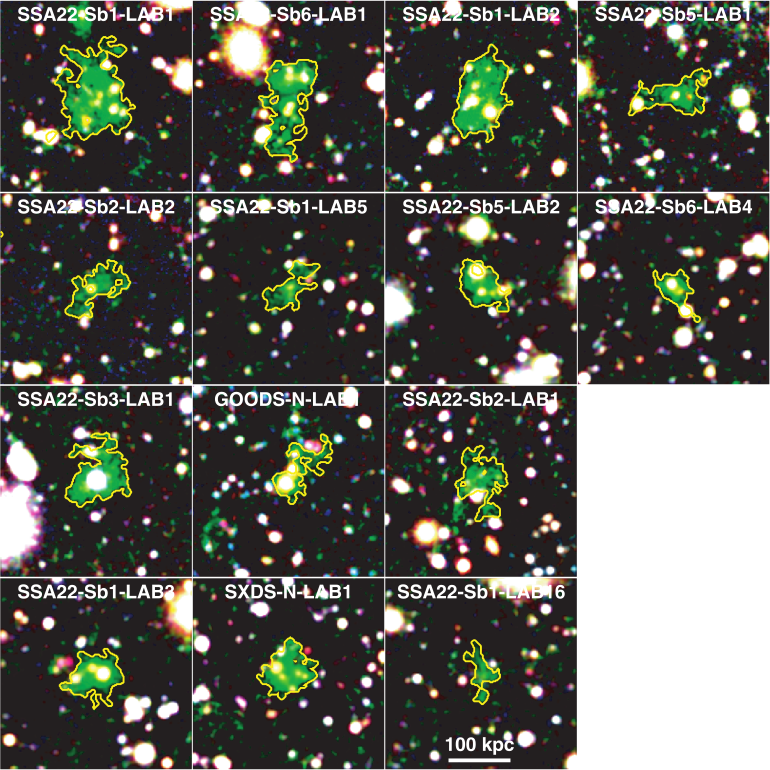
\includegraphics[width=\textwidth,height=\textheight,keepaspectratio]{figures/matsuda2011blobs.png}
    \caption{
        Surface brightness images that were presented in \citet{Matsuda2011}, which we present here to orient the reader to the sort of data we have as a ground truth.
    }
  \label{fig:matsuda2011blobs}
\end{figure*}

\section{The Definition of a Ly\texorpdfstring{$\alpha$}{a} Blob}
\label{sec:blob_definition}
There is no consensus definition of a Ly$\alpha$ blob in the literature.
We present in Table \ref{table:labs} a summary of recent papers papers aimed at observationally characterizing LABs, and quote their measurements of a few observed properties that could potentially be used to distinguish this class of objects from Lyman-alpha emitters.
As is evident, there is no clear luminosity threshold for a LAB definition.
Observations find luminosities ranging nearly $2$
orders of magnitude ($2\times10^{42}<L_{\rm Ly\alpha}<2.1\times10^{44}$ erg/s).
Similarly, there is no clear size definition.
Quoted diameters range from $30-200$ kpc, though the interpretation of this physical constraint is muddied by the fact that observations have a wide range of limiting surface brightness that range by over an order of magnitude in the literature.
Beyond this, the dispersion in this limiting surface brightness along with the amorphous morphology of Lyman-alpha blobs makes such size measurements difficult to interpret.
To further complicate matters, recent work by \citet{Wisotzki2018} has shown that with sufficient sensitivity nearly the whole sky is covered by Lyman-alpha.
Indeed, as we will demonstrate in this paper, the area enclosed by a Ly$\alpha$ blob is a strong function of the limiting surface brightness.

Going forward in this paper, we will adopt a notional threshold luminosity for blob definition of $L_{\rm Ly\alpha} > 10^{43}$ erg/s, with no size threshold.
This said, we will explore the impact of modifying these on our results.

\section{Theoretical Efforts to Date}

The source of Lyman-alpha emission from these objects is unclear, though there has been much theoretical work on them.

\citet{Furlanetto2005, Laursen2007, Cen2013, Geach2016, Gronke2017} have studied the contribution of star formation on the formation of LABs, and all conclude this source of Ly$\alpha$ can (or in the case of \citet{Cen2013} \emph{must}) power blobs.
Additionally, \citet{Cen2013} are able to reproduce an observed LAB luminosity-size relation.
This said, some of the previous work on the contribution of star formation relies on a simplified SFR-$L_{Ly\alpha}$ conversion based on the expected luminosity from case-B recombination.

There has also been extensive study of the contribution of Ly$\alpha$ emission due to collisionally excited neutral hydrogen \citep{Rosdahl2012, Fardal2001, Goerdt2010, Haiman2000, Faucher-Giguere2010}, or specifically the incoming streams of cooling IGM that are observed in some simulations at high redshift.
These works are able to reproduce the requisite Ly$\alpha$ luminosity to power a LAB, but sometimes have difficulty with the particular appearance of LABs in surface brightness maps.

Other authors have studied the effect of fluorescence from an external ionizing field such as a nearby or internal quasar \citep{Haiman2001} or the cosmological UV background or winds \citep{Furlanetto2005, Mas-Ribas2016}.
These authors find that an external ionizing radiation field can produce extended Ly$\alpha$ emission, but not quite at the surface brightnesses to produce a blob on its own.

Missing, to date, is a comprehensive model that considers all of these physical processes simultaneously.
This project is an attempt to provide just that.
We present a model for the formation and evolution of Ly$\alpha$ blobs by combining high-resolution cosmological zoom-in simulations (from the MassiveFIRE series of simulations) with ionization radiative transfer and Ly$\alpha$ radiative transfer.
We consider the necessary underlying physics to model Ly$\alpha$ production from ionized gas surrounding massive stars, collisional excitation (cooling), and fluourescence induced by other ionizing radiation fields (including AGN).
In \S~\ref{sec:methods}, we detail our numerical methodology; in \S~\ref{sec:evolution}, we describe the evolution of the Ly$\alpha$ luminosity from massive galaxies at high-redshift.
We follow this in \S~\ref{sec:origins} with an investigation into the dominant power sources of Ly$\alpha$ photons in massive galaxies and investigate the role of AGN in \S~\ref{sec:agn}.
We provide discussion in \S~\ref{sec:discussion}, and conclude in \S~\ref{sec:conclusions}.

    \begin{table*}
    \caption{An overview of Ly$\alpha$ properties for a sample of known LABs which we compare to our simulations}
    \centering
    \begin{tabular}{ | l | c | c | c | c | }
    \hline
        Publication & $z$ & $L_{\rm{Ly}\alpha}\ (\rm{erg}\ \rm{s}^{-1})$ & $\Sigma_{\rm{lim}}\ (\rm{erg}\ \rm{s}^{-1}\ \rm{cm}^{-2}\ \rm{arcsec}^{-2})$ & LAB size \\
    \hline

    \citet{Matsuda2004} & 3.1 & $1.1\times10^{44} - 5.8\times10^{42}$ & $2.2\times10^{-18}$ & 222 - 16 arcsec$^2$\\
    \hline

    \citet{Nilsson2006} & 3.16 &  $10^{43}$ & $3.7\times10^{-18}$ & 60 kpc diameter \\
    \hline

    \citet{Smith2007} & 2.83 & $2.1\times10^{44}$ & Unclear & 12 arcsec diameter \\
    \hline

    \citet{Ouchi2009} & 6.595 & $3.9\times10^{43}$ & $1.63\times10^{-18}$ & 3 arcseconds major axis \\
    \hline

    \citet{Yang2009} & 2.3 & $1.6-5.3\times10^{43}$ & $2.47\times10^{-18}$ & 25 arcsec$^{2}$\\
    \hline

    \citet{Matsuda2011} & 3.09 & 20.4 - 0.8 $\times10^{43}$ & $1.4\times10^{-18}$ & 28-181 arcsec$^{2}$\\
    \hline

    \citet{Steidel2011} & 2.65 & $6.57\times10^{43}$ & $\sim10^{-18}$ & 3 arcsec radius \\
    \hline

    \citet{Barger2012} & 0.977 & $10^{42.86}$ & Unclear & 500 arcsec$^{2}$ \\
    \hline

    \citet{Prescott2013} & 1.7-2.7 & $1.9\times10^{43}-2.6\times10^{42}$ & $9.33\times10^{-19}$ & 5.9-104 arcsec$^{2}$ \\
    \hline

    \citet{Caminha2016} & 3.118 & $1.9\times10^{42}$ & Unclear & 33 kpc \\
    \hline

    \citet{Badescu2017} & 2.3 & $0.9-1.3\times10^{43}$ & $2.1\times10^{-18}$ & 10-12 arcsec$^{2}$ \\ 
    \hline

    \citet{North2017} & 3.08 & $2.2\times10^{43}$ & $7.5\times10^{-18}$ & 3-4 arcseconds across\\
    \hline

    \citet{Shibuya2017} & 5.7-6.6 & $1.26\times10^{43} - 7.94\times10^{43}$ & $1.0 - 2.1\times10^{-17}$ & 2-3 arcsec$^{2}$\\
    \hline

    \end{tabular}
    \label{table:labs}
    \end{table*}


\section{Opening Remarks}
We are currently getting a publication through peer review which contains mostly the same results as are presented in this dissertation, but in that work we have attempted to tell a simple and coherent story.
In this dissertation we will try to elaborate as much as possible where things get complicated, and where our understanding fails us, propose future work on this topic.
% TODO: Cite the accompanying paper?

It also needs to be said that additional complication is added to this work by the currently-prevailing attitudes in this field about sharing data and code.
At the time of writing, we were not aware of any publicly-available codebase for Ly$\alpha$ radiative transfer.
This is particularly problematic for two reasons.
Firstly, anyone seeking to do such work must affiliate themselves with the owner of a closed-source codebase or invest a substantial amount time and effort in writing then debugging such a codebase.
We are eternally grateful for Aaron Smith for sharing and assisting in modifications to the Ly$\alpha$ MCRT codebase he wrote initially just for his own PhD work.
Without his generosity, this project could not have been completed in 3 short years, especially not by me, a student whose primary expertise at the time was on exoplanet radial velocity measurements.
We tried to write a Ly$\alpha$ MCRT code from scratch, and it did not go well.
Secondly, and perhaps more importantly we cannot compare our results and methodology in-depth to the work of other scientists who have come to conflicting conclusions.
We can only guess as to why.
Is it because the parts of our methodologies that we have shared differ?
Is it because of something we (and reviewers) thought not important enough to include in a paper?
Is it perhaps because one or both of our codebases contain bugs?
The prevailing attitude towards testing in astronomy is not good, and this is particularly problematic in this field.
In the absence of rigorous tests, we ask ``Does the output of this code make sense?''
But in a field with such extraordinary complexity where most things are nonlinear and a factor of 2 can be hard to notice, it is all too easy to explain away behavior that is in error.
We have certainly done this, multiple times.
The field needs to do better as a whole, and therefore we are releasing the Ly$\alpha$ MCRT code that he originally authored and we both maintained for the past years.
Of course we do not expect astronomers to descend on the codebase and make it beautiful and well-tested, but it is our sincere hope that we can save some wasted effort of code-writing and with more eyes can gradually fix any bugs that remain.

The situation with data is much harder.
The entirety of this work is analysis of 4 objects.
we wish that it could be more; one of the questions we've gotten from astronomers repeatedly is something like ``What can you tell us about the occurrence rate of these objects?''
One way to answer this question would be push many more cosmological zoom simulations through the pipeline we've built for this project.
Unfortunately, \red{the computational expense of running these zooms is significant} \red{WE KNOW WHERE TO GET THEM....WE HAVE THE CODE AND COMUTER TIME TO RUN THEM :) } we do not know where to get such zooms, and even if we did, the sheer size of these presents a serious problem.
The input data to this project is 20 TB.
We would love to push through 100 or so simulations, but the disk space and compute time for naively scaling up this project in such a manner would begin to rival the large cosmological simulations.
This could be done, but the scale that this project has remained at is comfortably within the scope of everyday data management and thus no time in this project was budgeted for solving big data and big compute problems; if the project were scaled up significantly that may have to change.
But even in the presence of a way to move and store that much data, we would need to actually get it which is not really possible in a field with a prevailing closed-source, closed-data mindset.
We would like to offer up solutions to all these problems; but unfortunately cannot in this project, and so this short section is just an attempt to raise some awareness of the non-science problems we have faced.
